% Options for packages loaded elsewhere
% Options for packages loaded elsewhere
\PassOptionsToPackage{unicode}{hyperref}
\PassOptionsToPackage{hyphens}{url}
%
\documentclass[
  ignorenonframetext,
]{beamer}
\newif\ifbibliography
\usepackage{pgfpages}
\setbeamertemplate{caption}[numbered]
\setbeamertemplate{caption label separator}{: }
\setbeamercolor{caption name}{fg=normal text.fg}
\beamertemplatenavigationsymbolsempty
% remove section numbering
\setbeamertemplate{part page}{
  \centering
  \begin{beamercolorbox}[sep=16pt,center]{part title}
    \usebeamerfont{part title}\insertpart\par
  \end{beamercolorbox}
}
\setbeamertemplate{section page}{
  \centering
  \begin{beamercolorbox}[sep=12pt,center]{section title}
    \usebeamerfont{section title}\insertsection\par
  \end{beamercolorbox}
}
\setbeamertemplate{subsection page}{
  \centering
  \begin{beamercolorbox}[sep=8pt,center]{subsection title}
    \usebeamerfont{subsection title}\insertsubsection\par
  \end{beamercolorbox}
}
% Prevent slide breaks in the middle of a paragraph
\widowpenalties 1 10000
\raggedbottom
\AtBeginPart{
  \frame{\partpage}
}
\AtBeginSection{
  \ifbibliography
  \else
    \frame{\sectionpage}
  \fi
}
\AtBeginSubsection{
  \frame{\subsectionpage}
}
\usepackage{iftex}
\ifPDFTeX
  \usepackage[T1]{fontenc}
  \usepackage[utf8]{inputenc}
  \usepackage{textcomp} % provide euro and other symbols
\else % if luatex or xetex
  \usepackage{unicode-math} % this also loads fontspec
  \defaultfontfeatures{Scale=MatchLowercase}
  \defaultfontfeatures[\rmfamily]{Ligatures=TeX,Scale=1}
\fi
\usepackage{lmodern}

\ifPDFTeX\else
  % xetex/luatex font selection
\fi
% Use upquote if available, for straight quotes in verbatim environments
\IfFileExists{upquote.sty}{\usepackage{upquote}}{}
\IfFileExists{microtype.sty}{% use microtype if available
  \usepackage[]{microtype}
  \UseMicrotypeSet[protrusion]{basicmath} % disable protrusion for tt fonts
}{}
\makeatletter
\@ifundefined{KOMAClassName}{% if non-KOMA class
  \IfFileExists{parskip.sty}{%
    \usepackage{parskip}
  }{% else
    \setlength{\parindent}{0pt}
    \setlength{\parskip}{6pt plus 2pt minus 1pt}}
}{% if KOMA class
  \KOMAoptions{parskip=half}}
\makeatother


\usepackage{longtable,booktabs,array}
\usepackage{calc} % for calculating minipage widths
\usepackage{caption}
% Make caption package work with longtable
\makeatletter
\def\fnum@table{\tablename~\thetable}
\makeatother
\usepackage{graphicx}
\makeatletter
\newsavebox\pandoc@box
\newcommand*\pandocbounded[1]{% scales image to fit in text height/width
  \sbox\pandoc@box{#1}%
  \Gscale@div\@tempa{\textheight}{\dimexpr\ht\pandoc@box+\dp\pandoc@box\relax}%
  \Gscale@div\@tempb{\linewidth}{\wd\pandoc@box}%
  \ifdim\@tempb\p@<\@tempa\p@\let\@tempa\@tempb\fi% select the smaller of both
  \ifdim\@tempa\p@<\p@\scalebox{\@tempa}{\usebox\pandoc@box}%
  \else\usebox{\pandoc@box}%
  \fi%
}
% Set default figure placement to htbp
\def\fps@figure{htbp}
\makeatother





\setlength{\emergencystretch}{3em} % prevent overfull lines

\providecommand{\tightlist}{%
  \setlength{\itemsep}{0pt}\setlength{\parskip}{0pt}}



 


\makeatletter
\@ifpackageloaded{tcolorbox}{}{\usepackage[skins,breakable]{tcolorbox}}
\@ifpackageloaded{fontawesome5}{}{\usepackage{fontawesome5}}
\definecolor{quarto-callout-color}{HTML}{909090}
\definecolor{quarto-callout-note-color}{HTML}{0758E5}
\definecolor{quarto-callout-important-color}{HTML}{CC1914}
\definecolor{quarto-callout-warning-color}{HTML}{EB9113}
\definecolor{quarto-callout-tip-color}{HTML}{00A047}
\definecolor{quarto-callout-caution-color}{HTML}{FC5300}
\definecolor{quarto-callout-color-frame}{HTML}{acacac}
\definecolor{quarto-callout-note-color-frame}{HTML}{4582ec}
\definecolor{quarto-callout-important-color-frame}{HTML}{d9534f}
\definecolor{quarto-callout-warning-color-frame}{HTML}{f0ad4e}
\definecolor{quarto-callout-tip-color-frame}{HTML}{02b875}
\definecolor{quarto-callout-caution-color-frame}{HTML}{fd7e14}
\makeatother
\makeatletter
\@ifpackageloaded{caption}{}{\usepackage{caption}}
\AtBeginDocument{%
\ifdefined\contentsname
  \renewcommand*\contentsname{Table of contents}
\else
  \newcommand\contentsname{Table of contents}
\fi
\ifdefined\listfigurename
  \renewcommand*\listfigurename{List of Figures}
\else
  \newcommand\listfigurename{List of Figures}
\fi
\ifdefined\listtablename
  \renewcommand*\listtablename{List of Tables}
\else
  \newcommand\listtablename{List of Tables}
\fi
\ifdefined\figurename
  \renewcommand*\figurename{Figure}
\else
  \newcommand\figurename{Figure}
\fi
\ifdefined\tablename
  \renewcommand*\tablename{Table}
\else
  \newcommand\tablename{Table}
\fi
}
\@ifpackageloaded{float}{}{\usepackage{float}}
\floatstyle{ruled}
\@ifundefined{c@chapter}{\newfloat{codelisting}{h}{lop}}{\newfloat{codelisting}{h}{lop}[chapter]}
\floatname{codelisting}{Listing}
\newcommand*\listoflistings{\listof{codelisting}{List of Listings}}
\makeatother
\makeatletter
\makeatother
\makeatletter
\@ifpackageloaded{caption}{}{\usepackage{caption}}
\@ifpackageloaded{subcaption}{}{\usepackage{subcaption}}
\makeatother

\usepackage{bookmark}
\IfFileExists{xurl.sty}{\usepackage{xurl}}{} % add URL line breaks if available
\urlstyle{same}
\hypersetup{
  pdftitle={Résolution des modèles DSGE},
  pdfauthor={Pablo Winant},
  hidelinks,
  pdfcreator={LaTeX via pandoc}}


\title{Résolution des modèles DSGE}
\subtitle{Macro II - Fluctuations - ENSAE, 2024-2025}
\author{Pablo Winant}
\date{2025-03-12}

\begin{document}
\frame{\titlepage}


\section{Introduction}\label{introduction}

\begin{frame}{}
\phantomsection\label{section}
\begin{columns}[T]
\begin{column}{0.8\linewidth}
Quelle est la principale spécificité de la modélisation économique ?

En (macro)économie, nous \emph{modélisons} le comportement des agents
économiques en spécifiant :

\begin{itemize}
\tightlist
\item
  leur objectif \[\max_{c_t} E_t \sum_{s\geq t} \beta^s U(c_s)\]
  \[\max \pi_t\] \[\cdots\]
\item
  leurs contraintes (contrainte budgétaire, environnement éco\ldots)
\end{itemize}
\end{column}

\begin{column}{0.2\linewidth}
\pandocbounded{
\includegraphics[keepaspectratio]{assets/lucifer.jpg}}
\end{column}
\end{columns}

\pause

Cela a des implications importantes :

\begin{itemize}
\tightlist
\item
  les modèles macro sont orientés vers le futur (\emph{forward looking})

  \begin{itemize}
  \tightlist
  \item
    ils reposent sur les anticipations
  \end{itemize}
\item
  les modèles macro doivent être \textbf{résolus}
\end{itemize}

Dans de nombreux cas, il n'existe pas de forme fermée pour la solution
-\textgreater{} il faut des \emph{techniques numériques}
\end{frame}

\begin{frame}{Dynare}
\phantomsection\label{dynare}
\begin{columns}[T]
\begin{column}{0.6\linewidth}
\begin{itemize}[<+->]
\tightlist
\item
  1996 : Michel Juillard crée un logiciel open source pour résoudre des
  modèles DSGE

  \begin{itemize}[<+->]
  \tightlist
  \item
    DSGE : Dynamic Stochastic General Equilibrium
  \item
    généralement résolus autour d'un état stationnaire
  \end{itemize}
\item
  Aujourd'hui, environ 10 contributeurs.

  \begin{itemize}[<+->]
  \tightlist
  \item
    \(+\) des power users qui ont contribué au code
  \end{itemize}
\end{itemize}

\begin{itemize}
\tightlist
\item
  Il a été largement adopté :

  \begin{itemize}
  \tightlist
  \item
    premières versions sous Gauss
  \item
    puis Matlab/Octave/Scilab
  \item
    dernière version en Julia
  \item
    \ldots{} et Python (voir
    \href{https://www.mosphere.fr/ae2e6_models/voici/tree/index.html}{dyno
    🦖})
  \end{itemize}
\end{itemize}
\end{column}

\begin{column}{0.4\linewidth}
\begin{figure}[H]

{\centering \pandocbounded{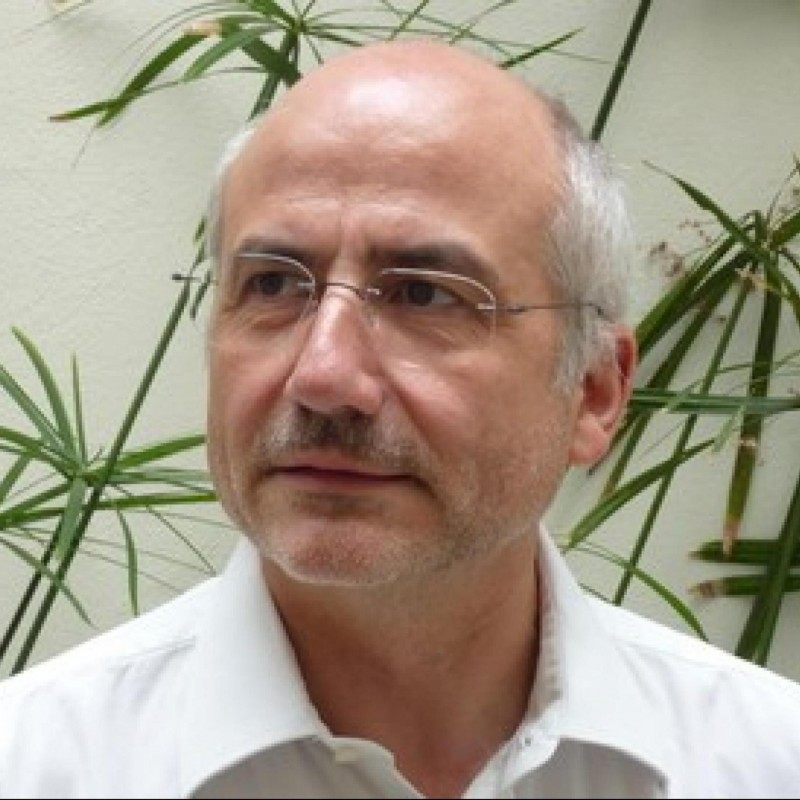
\includegraphics[keepaspectratio]{assets/michel.jpeg}}

}

\caption{Michel Juillard}

\end{figure}%
\end{column}
\end{columns}
\end{frame}

\begin{frame}{Modèles DSGE dans les institutions}
\phantomsection\label{moduxe8les-dsge-dans-les-institutions}
Aujourd'hui, la plupart des modèles DSGE développés dans les
institutions ont une version Dynare (FMI/GIMF, CE/Quest, BCE/,
NYFed/FRBNY)

\begin{itemize}
\tightlist
\item
  ils sont généralement basés sur le \emph{modèle de taille
  intermédiaire} de Smets \& Wouters (10 équations)
\item
  mais ils ont beaucoup grandi (\textgreater\textgreater100 équations)
\end{itemize}

\pause

Les institutions, portées par les chercheurs, diversifient leurs modèles

\begin{itemize}
\tightlist
\item
  Modèles semi-structurels
\item
  Modèles d'équilibre général calculable
\item
  Modèles de réseaux
\item
  Modèles à agents
\item
  Modèles à agents hétérogènes
\end{itemize}
\end{frame}

\begin{frame}{Plan}
\phantomsection\label{plan}
Fournir une courte introduction à la modélisation DSGE :

\begin{itemize}
\tightlist
\item
  Comment les modèles sont résolus (aujourd'hui)
\item
  Petite économie ouverte (aka modèle IRBC)
\item
  Hétérogénéité
\item
  Intermédiation financière
\end{itemize}

Au passage, nous discuterons de certaines tendances
\end{frame}

\section{Résolution d'un modèle}\label{ruxe9solution-dun-moduxe8le}

\begin{frame}{Modèle}
\phantomsection\label{moduxe8le}
Une représentation très concise d'un modèle

\[\mathbb{E}_t \left[ f(y_{t+1}, y_t, y_{t-1}, \epsilon_t) \right]= 0\]

\begin{columns}[T]
\begin{column}{0.48\linewidth}
Le \textbf{problème} :

\begin{itemize}
\tightlist
\item
  \(y_t\in\mathbb{R}^n\) : le vecteur des variables endogènes
\item
  \(\epsilon_t\in\mathbb{R}^{n_e}\) : le vecteur des variables exogènes

  \begin{itemize}
  \tightlist
  \item
    on suppose que \(\epsilon_t\) est un processus gaussien centré
  \end{itemize}
\item
  \(f: \mathbb{R}^n\rightarrow \mathbb{R}^n\) : les équations du modèle
\end{itemize}
\end{column}

\begin{column}{0.48\linewidth}
La \textbf{solution} :

\begin{itemize}
\tightlist
\item
  \(g\) telle que \[\forall t, y_t = g(y_{t-1},\epsilon_t)\]
\end{itemize}
\end{column}
\end{columns}

\note{La situation est différente lorsqu'on réalise une simulation en
prévision parfaite.}
\end{frame}

\begin{frame}[fragile]{Le timing des équations}
\phantomsection\label{le-timing-des-uxe9quations}
\begin{tcolorbox}[enhanced jigsaw, leftrule=.75mm, opacitybacktitle=0.6, rightrule=.15mm, colback=white, coltitle=black, bottomtitle=1mm, colbacktitle=quarto-callout-tip-color!10!white, title=\textcolor{quarto-callout-tip-color}{\faLightbulb}\hspace{0.5em}{Tip}, colframe=quarto-callout-tip-color-frame, arc=.35mm, left=2mm, toprule=.15mm, titlerule=0mm, breakable, toptitle=1mm, opacityback=0, bottomrule=.15mm]

Dans un modefile dynare, les équations du modèle sont codées dans le
bloc \texttt{model;\ ...\ ;\ end;}.

La variable \(v_t\) (resp \(v_{t-1}\), \(v_{t+1}\)) est notée \texttt{v}
ou \texttt{v(0)} (resp \texttt{v(-1)}, \texttt{v(+1)}).

\end{tcolorbox}

\textbf{Convention générale de timing}

La nouvelle information arrive avec les innovations \(\epsilon_t\).

À la date \(t\), l'ensemble d'information est engendré par
\(\mathcal{F}_t = \mathcal{F} (\cdots, \epsilon_{t-3}, \epsilon_{t-2}, \epsilon_{t-1}, \epsilon_t)\)

Par convention, \emph{une variable endogène a l'indice \(t\) si elle est
connue pour la première fois à la date \(t\)}.

\pause

Plusieurs \textbf{types de variables} selon leur apparition dans le
modèle :

\begin{itemize}
\tightlist
\item
  variable de saut : apparaît en \(t\) ou \(t+1\)
\item
  variable prédéterminée : apparaît en \(t-1\) et \(t\) (éventuellement
  \(t+1\))
\item
  variable statique : apparaît seulement en \(t\)

  \begin{itemize}
  \tightlist
  \item
    peut être exprimée en fonction d'autres variables
  \end{itemize}
\end{itemize}
\end{frame}

\begin{frame}{Le timing des équations}
\phantomsection\label{le-timing-des-uxe9quations-1}
\begin{block}{Exemple}
\phantomsection\label{exemple}
Avec les conventions de timing de Dynare :

\begin{itemize}
\item
  Écrire la fonction de production dans le modèle RBC
\item
  Écrire la loi de mouvement du capital \(k\), avec un taux de
  dépréciation \(\delta\) et l'investissement \(i\)

  \begin{itemize}
  \tightlist
  \item
    quand le capital est-il connu ?
  \item
    quand l'investissement est-il connu ?
  \end{itemize}
\item
  Ajouter un choc multiplicatif d'efficacité de l'investissement
  \(\chi_t\). Supposer qu'il suit un \(AR1\) piloté par l'innovation
  \(\eta_t\) et l'autocorrélation \(\rho_{\chi}\)

  \begin{itemize}
  \tightlist
  \item
    comment écrivez-vous la loi de mouvement du capital ?
  \end{itemize}
\end{itemize}
\end{block}
\end{frame}

\begin{frame}[fragile]{État stationnaire}
\phantomsection\label{uxe9tat-stationnaire}
L'état stationnaire déterministe vérifie :

\[f(\overline{y},\overline{y}, \overline{y}, 0)= 0\]

Souvent, il existe une solution en forme fermée.

Sinon, il faut recourir à un solveur numérique pour résoudre

\[\overline{y}\rightarrow f(\overline{y},\overline{y}, \overline{y}, 0)\]

\begin{tcolorbox}[enhanced jigsaw, leftrule=.75mm, opacitybacktitle=0.6, rightrule=.15mm, colback=white, coltitle=black, bottomtitle=1mm, colbacktitle=quarto-callout-tip-color!10!white, title=\textcolor{quarto-callout-tip-color}{\faLightbulb}\hspace{0.5em}{Tip}, colframe=quarto-callout-tip-color-frame, arc=.35mm, left=2mm, toprule=.15mm, titlerule=0mm, breakable, toptitle=1mm, opacityback=0, bottomrule=.15mm]

Dans dynare, les valeurs d'état stationnaire sont fournies dans le bloc
\texttt{steadystate\_model;\ ...\ ;\ end;}. On peut vérifier qu'elles
sont correctes avec l'instruction \texttt{check;}.

Pour trouver numériquement l'état stationnaire : \texttt{steady;}.

\end{tcolorbox}
\end{frame}

\begin{frame}{Le système implicite}
\phantomsection\label{le-systuxe8me-implicite}
En remplaçant la solution \[y_t = \color{red}{g}(y_{t-1},\epsilon_t)\]
dans le système
\[\mathbb{E}_t \left[ f(y_{t+1}, y_t, y_{t-1}, \epsilon_t) \right]= 0\]

on obtient :

\[\mathbb{E}_t \left[ f(\color{red}{g}(\color{red}{g}(y_{t-1},\epsilon_{t}),\epsilon_{t+1}), \color{red}{g}(y_{t-1},\epsilon_t), y_{t-1}, \epsilon_t) \right]= 0\]

C'est une équation qui définit implicitement la fonction
\(\color{red}{g}()\)
\end{frame}

\begin{frame}{L'espace d'état}
\phantomsection\label{lespace-duxe9tat}
\[\mathbb{E}_t \left[ f(\color{red}{g}(\color{red}{g}(y_{t-1},\epsilon_{t}),\epsilon_{t+1}), \color{red}{g}(y_{t-1},\epsilon_t), y_{t-1}, \epsilon_t) \right]= 0\]

Dans cette expression, \(y_{t-1},\epsilon_t\) est l'espace d'état :

\begin{itemize}
\tightlist
\item
  il contient toute l'information disponible en \(t\) pour prédire
  l'évolution future de \((y_s)_{s\geq t}\)
\end{itemize}

\pause

En supprimant les indices temporels, l'équation doit être satisfaite
pour toute réalisation de \((y,\epsilon)\)
\[\forall (y,\epsilon)\  \Phi(\color{red}{g})(y,\epsilon) = \mathbb{E}_{\epsilon'} \left[ f(\color{red}{g}(\color{red}{g}(y,\epsilon),\epsilon'), \color{red}{g}(y,\epsilon), y, \epsilon) \right]= 0\]

C'est une équation fonctionnelle \(\Phi(\color{red}{g})=0\)
\end{frame}

\begin{frame}{Chocs anticipés}
\phantomsection\label{chocs-anticipuxe9s}
Approximation du premier ordre :

\begin{itemize}
\tightlist
\item
  Supposer \(|\epsilon|<<1\),\(|\epsilon'|<<1\)
\end{itemize}

Effectuer un développement de Taylor par rapport au choc futur :

\begin{align}
 & & \mathbb{E}_{\color{green}{\epsilon'}} \left[ f(g(g(y,\epsilon),\color{green}{\epsilon'}), g(y,\epsilon), y, \epsilon) \right]  \\
= & &  \mathbb{E}_{\color{green}{\epsilon'}}\left[ f(g(g(y,\epsilon),0), g(y,\epsilon), y, \epsilon) \right] \\ 
  & & +  \mathbb{E}_{\color{green}{\epsilon'}} \left[ f^{\prime}_{y_{t+1}}(g(g(y,\epsilon),0), g(y,\epsilon), y, \epsilon) g^{\prime}_{\epsilon} \color{green}{\epsilon'}\right] + o(\epsilon^{\prime}) \\
\approx & & f(g(g(y,\epsilon),0), g(y,\epsilon), y, \epsilon)
\end{align}

\pause

On utilise le fait que
\(\mathbb{E}\left[ \epsilon^{\prime}\right] = 0\).

Au premier ordre, les chocs anticipés ne jouent aucun rôle.

Pour capturer les comportements de précaution (comme les primes de
risque), il faut augmenter l'ordre d'approximation.
\end{frame}

\begin{frame}{Perturbation du premier ordre}
\phantomsection\label{perturbation-du-premier-ordre}
Il nous reste le système :

\[F(y,\epsilon) = f(g(g(y,\epsilon),0), g(y,\epsilon), y, \epsilon) = 0\]

Une variante du \emph{théorème des fonctions implicites} donne alors
l'existence d'une première approximation de \(g\) :

\[g(y,\epsilon) = \overline{y} + g^{\prime}_{y} (y-\overline{y}) + g^{\prime}_e \epsilon_t \]

\pause

Les quantités inconnues \(g^{\prime}_y\), et \(g^{\prime}_e\) sont
obtenues avec la \emph{méthode des coefficients indéterminés}. On
injecte la première approximation dans le système et on écrit les
conditions \[F^{\prime}_y(\overline{y}, 0) = 0\]
\[F^{\prime}_\epsilon(\overline{y}, 0) = 0\]
\end{frame}

\begin{frame}{Calcul de \(g^{\prime}_y\)}
\phantomsection\label{calcul-de-gprime_y}
Rappel du système :
\[F(y,\epsilon) = f(g(g(y,\epsilon),0), g(y,\epsilon), y, \epsilon) = 0\]

On a
\[F^{\prime}_y(\overline{y}, 0) = f^{\prime}_{y_{t+1}} g^{\prime}_y g^{\prime}_y + f^{\prime}_{y_{t}} g^{\prime}_y + f^{\prime}_{y_{t-1}} = 0 \]

\pause

\(g^{\prime}_y\) est la solution d'une équation de Riccati spécifique
\[A X^2 + B X + C\] où \(A,B,C\) et \(X=g^{\prime}_y\) sont des matrices
carrées \(\in \mathbb{R}^n \times \mathbb{R}^n\)
\end{frame}

\begin{frame}{Modèle déterministe du premier ordre}
\phantomsection\label{moduxe8le-duxe9terministe-du-premier-ordre}
Faisons une pause pour observer le modèle déterministe du premier ordre
: \[A X^2 + B X + C\]

D'après notre intuition en dimension 1, on sait qu'il doit y avoir
plusieurs solutions

\begin{itemize}
\tightlist
\item
  comment les trouver ?
\item
  comment sélectionner les bonnes ?
\end{itemize}

En l'absence de chocs, la dynamique du modèle est donnée par
\[y_t = X y_{t-1}\]

Quelle est la condition pour que le modèle soit stationnaire ?

\pause

-\textgreater{} la plus grande valeur propre de \(X\) doit être
inférieure à 1

\note{Développer l'intuition en dimension 1.}
\end{frame}

\begin{frame}{Multiplicité des solutions}
\phantomsection\label{multiplicituxe9-des-solutions}
On peut montrer que le système est associé à \(2 n\) valeurs propres
généralisées :

\[|\lambda_1| \leq \cdots \leq |\lambda_{2 n}|\]

Pour chaque choix \(C\) de \(n\) valeurs propres (\(|C|=n\)), une
solution récursive spécifique \(X_C\) peut être \emph{construite}. Elle
a pour valeurs propres \(C\).

\pause

Cela donne au moins
\(\left(\begin{matrix} 2 n \\ n \end{matrix}\right)\) combinaisons
différentes.

\pause

Un modèle est bien défini lorsqu'il existe \textbf{exactement une
solution non divergente}.

Ceci est équivalent à :

\[|\lambda_1| \leq \cdots \leq |\lambda_{n}| \leq 1 < |\lambda_{n+1}| \leq \cdots \leq |\lambda_{2 n}|\]
\end{frame}

\begin{frame}{Exemple 1}
\phantomsection\label{exemple-1}
Inflation orientée vers le futur :

\[\pi_t = \alpha \pi_{t+1}\] avec \(\alpha<1\).

Le modèle est-il bien défini ?

\pause

On peut réécrire le système :

\[\alpha \pi_{t+1} - \pi_t + 0 \pi_{t-1}  = 0\]

ou

\[\pi_{t+1} - \left(\frac{1}{\alpha} + 0 \right)\pi_t + \left(\frac{1}{\alpha} 0\right) \pi_{t-1} = 0\]

\pause

Les valeurs propres généralisées sont \(0\leq 1 < \frac{1}{\alpha}\).

\pause

La solution stable unique est \(\pi_t=0 \pi_{t-1}\)
\end{frame}

\begin{frame}{Exemple 2}
\phantomsection\label{exemple-2}
Équation d'accumulation de dette par un agent rationnel :

\[b_{t+1} - (1+\frac{1}{\beta}) b_t + \frac{1}{\beta} b_{t-1} = 0\]

Le modèle est-il bien défini ?

\pause

Deux valeurs propres généralisées
\(\lambda_1=1 < \lambda_2=\frac{1}{\beta}\)

\pause

La solution unique non divergente est \(b_t = b_{t-1}\).

\begin{itemize}
\tightlist
\item
  c'est une \emph{racine unitaire} : toute déviation initiale de
  \(b_{t-1}\) a des effets persistants
\end{itemize}
\end{frame}

\begin{frame}{Exemple 3}
\phantomsection\label{exemple-3}
Processus de productivité : \[z_t = \rho z_{t-1}\] avec \(\rho<1\) :
{bien défini}

\pause

Dans ce cas, il existe une valeur propre infinie cachée \(\infty\)
associée à \(z_{t+1}\).

\pause

Pour voir pourquoi, considérer le système associé aux valeurs propres
\(m\) et \(\rho\) : \[z_{t+1} - (m+\rho) z_t + m \rho z_{t-1} = 0\]

\[\frac{1}{m} z_{t+1} - (1+\frac{\rho}{m}) z_t + \rho z_{t-1} = 0\]

Ce qui correspond au modèle initial quand \(m=\infty\)

\pause

Les valeurs propres généralisées sont
\(\lambda_1 = \rho \leq 1 < \lambda_2 = \infty\)

Plus généralement, toute variable qui n'apparaît pas en \(t+1\) crée une
valeur propre généralisée infinie.
\end{frame}

\begin{frame}{Un critère de bonne définition}
\phantomsection\label{un-crituxe8re-de-bonne-duxe9finition}
En regardant à nouveau la liste des valeurs propres, on met de côté les
valeurs infinies.

Le modèle est bien spécifié ssi on peut ordonner les valeurs propres
comme suit :

\[|\lambda_1| \leq \cdots \leq |\lambda_{n}| \leq 1 < |\lambda_{n+1}| \leq \cdots  |\lambda_{n+k}| \leq \underbrace{|\lambda_{n+k+1}| \cdots \leq |\lambda_{2 n}|}_{\text{valeurs propres infinies}}\]

\begin{tcolorbox}[enhanced jigsaw, leftrule=.75mm, opacitybacktitle=0.6, rightrule=.15mm, colback=white, coltitle=black, bottomtitle=1mm, colbacktitle=quarto-callout-note-color!10!white, title=\textcolor{quarto-callout-note-color}{\faInfo}\hspace{0.5em}{Critère de Blanchard-Kahn}, colframe=quarto-callout-note-color-frame, arc=.35mm, left=2mm, toprule=.15mm, titlerule=0mm, breakable, toptitle=1mm, opacityback=0, bottomrule=.15mm]

Le modèle satisfait le critère de Blanchard-Kahn si le nombre de valeurs
propres supérieures à un est exactement égal au nombre de variables
\emph{apparaissant} en \(t+1\).

Dans ce cas, le modèle est bien défini.

\end{tcolorbox}
\end{frame}

\begin{frame}{Calcul de la solution}
\phantomsection\label{calcul-de-la-solution}
Il existe plusieurs méthodes classiques pour calculer la solution de
l'équation algébrique de Riccati : \[A X^2+ B X + C=0\]

\begin{itemize}
\tightlist
\item
  décomposition qz

  \begin{itemize}
  \tightlist
  \item
    traditionnellement utilisée dans la littérature DSGE depuis Chris
    Sims
  \item
    un peu contre-intuitive
  \end{itemize}
\item
  réduction cyclique

  \begin{itemize}
  \tightlist
  \item
    nouveau défaut dans dynare, mieux adaptée aux grands modèles
  \end{itemize}
\item
  itération temporelle linéaire cf @sec:linear\_time\_iteration

  \begin{itemize}
  \tightlist
  \item
    conceptuellement très simple
  \end{itemize}
\end{itemize}
\end{frame}

\begin{frame}{Calcul de \(g^{\prime}_{e}\)}
\phantomsection\label{calcul-de-gprime_e}
Maintenant que nous avons \(g^{\prime}_y\), comment obtenir
\(g^{\prime}_{e}\) ?

Rappel :
\[F(y,\epsilon) = f(g(g(y,\epsilon),0), g(y,\epsilon), y, \epsilon) = 0\]

On a
\[F^{\prime}_e(\overline{y}, 0) =  f^{\prime}_{y_{t+1}}  g^{\prime}_y  g^{\prime}_e + f^{\prime}_{y_{t}} g^{\prime}_e + f^{\prime}_{\epsilon_t} = 0 \]

Maintenant c'est facile :

\[g^{\prime}_e = - (f^{\prime}_{y_{t+1}}  g^{\prime}_y + f^{\prime}_{y_{t}} )^{-1}  f^{\prime}_{\epsilon_t} = 0 \]
\end{frame}

\begin{frame}{La solution du modèle}
\phantomsection\label{la-solution-du-moduxe8le}
Le résultat de la résolution du modèle :
\[y_t = g_y y_{t-1} + g_e \epsilon_t\]

C'est un AR1, piloté par le choc exogène \(\epsilon_t\).

\pause

Comme c'est une structure bien connue, on peut analyser le modèle avec

\begin{itemize}
\tightlist
\item
  des fonctions de réponse impulsionnelle
\item
  des simulations stochastiques
\end{itemize}

\pause

Puis, pour comparer le modèle aux données, on calcule

\begin{itemize}
\tightlist
\item
  les moments implicites :

  \begin{itemize}
  \tightlist
  \item
    covariances, autocorrélation
  \end{itemize}
\item
  la vraisemblance
\end{itemize}

Optimiser l'ajustement aux données s'appelle l'estimation du
\emph{modèle}
\end{frame}

\section{Conclusion}\label{sec-conclusion}

\begin{frame}{Que faire avec la solution}
\phantomsection\label{que-faire-avec-la-solution}
La solution d'un modèle trouvée par Dynare a une forme particulièrement
simple : un AR1

\begin{itemize}
\tightlist
\item
  \(y_t = X y_{t-1} + Y \epsilon_t\)
\item
  où les covariances \(\Sigma\) de \(\epsilon_t\) peuvent être choisies
  par le modélisateur
\end{itemize}

\pause

Avec cette solution, on peut (cf prochain TD)

\begin{itemize}
\tightlist
\item
  calculer des moments (conditionnels et inconditionnels)
\item
  réaliser des simulations stochastiques, fonctions de réponse
  impulsionnelle
\end{itemize}

\pause
\end{frame}

\begin{frame}{Aller plus loin}
\phantomsection\label{aller-plus-loin}
Amener le modèle aux données avec Dynare

\begin{itemize}
\tightlist
\item
  ``estimer'' le modèle : calculer la vraisemblance d'une solution et la
  maximiser en choisissant les bons paramètres
\item
  ``identifier'' les chocs dans les données
\end{itemize}

Autres fonctions

\begin{itemize}
\tightlist
\item
  approximation d'ordre supérieur
\item
  simulations en prévision parfaite (non linéaires)
\item
  plan de Ramsey
\item
  politique discrétionnaire
\item
  \ldots{}
\end{itemize}
\end{frame}

\begin{frame}{À venir}
\phantomsection\label{uxe0-venir}
\pandocbounded{
\includegraphics[keepaspectratio]{assets/ea0.jpg}}

De nombreux modèles
\end{frame}

\section{Annexe : itération temporelle
linéaire}\label{sec:linear_time_iteration}

\begin{frame}{Itération temporelle linéaire}
\phantomsection\label{ituxe9ration-temporelle-linuxe9aire}
Rappel du système à résoudre :
\[F(y,\epsilon) = f(g(g(y,\epsilon),0), g(y,\epsilon), y, \epsilon) = 0\]

mais supposons maintenant que les règles de décision aujourd'hui et
demain soient différentes :

\begin{itemize}
\tightlist
\item
  aujourd'hui :
  \(y_t = g(y_{t-1}, \epsilon_t) = \overline{y} + X y_{t-1} + g_y \epsilon_t\)
\item
  demain :
  \(y_{t+1} = \tilde{g}(y_t, \epsilon_{t+1}) = \overline{y} + \tilde{X} y_{t-1} + \tilde{g}_y \epsilon_t\)
\end{itemize}

L'équation de Riccati s'écrit alors :

\[A \tilde{X} X + B X + C = 0\]
\end{frame}

\begin{frame}{Itération temporelle linéaire (2)}
\phantomsection\label{ituxe9ration-temporelle-linuxe9aire-2}
L'algorithme d'itération temporelle linéaire consiste à résoudre la
règle de décision \(X\) aujourd'hui en fonction de la règle de décision
demain \(\tilde{X}\).

Cela correspond à la formule simple :

\[X = -(A\tilde{X} + B)^{-1} C\]

Et l'algorithme complet peut être décrit ainsi :

\begin{itemize}
\tightlist
\item
  choisir \(X_0\)
\item
  pour tout \(X_n\), calculer \(X_{n+1} = T(X_n) = -(A X_n + B)^{-1} C\)

  \begin{itemize}
  \tightlist
  \item
    répéter jusqu'à convergence
  \end{itemize}
\end{itemize}
\end{frame}

\begin{frame}{Itération temporelle linéaire (3)}
\phantomsection\label{ituxe9ration-temporelle-linuxe9aire-3}
On peut montrer qu'en partant d'une valeur initiale aléatoire,
l'algorithme d'itération temporelle linéaire converge vers la solution
\(X\) de plus petit module :

\[\underbrace{|\lambda_1| \leq \cdots  \leq |\lambda_n|}_{\text{Valeurs propres sélectionnées}} \leq |\lambda_{n+1}|\cdots \leq |\lambda_{2n}|\]

Autrement dit, il trouve la bonne solution lorsque le modèle est bien
spécifié.

Comment vérifier qu'il est bien spécifié ?

\begin{itemize}
\tightlist
\item
  \(\lambda_n\) est la plus grande valeur propre de la solution \(X\)
\item
  et pour \(\lambda_{n+1}\) ?

  \begin{itemize}
  \tightlist
  \item
    \(\frac{1}{\lambda_{n+1}}\) est la plus grande valeur propre de
    \((AX+B)^{-1}A\)
  \end{itemize}
\end{itemize}
\end{frame}

\begin{frame}{Itération temporelle linéaire (4)}
\phantomsection\label{ituxe9ration-temporelle-linuxe9aire-4}
Définir \[M(\lambda) = A\lambda^2 + B \lambda + C\]

Pour toute solution \(X\), \(M(\lambda)\) peut être factorisée comme :
\footnote<.->[frame]{Cas particulier du théorème de Bezout. Facile à
  vérifier dans ce cas}

\[M(\lambda)=(\lambda A + A X + B)(\lambda I -X)\]

et

\[det(M(\lambda)) = \underbrace{det(\lambda A + A X + B)}_{Q(\lambda)}det(\lambda I -X)\]

Par construction, \(Q(\lambda)\) est un polynôme dont les racines sont
celles qui ne sont pas sélectionnées par la solution,
c.-à-d.~\(\Lambda\setminus Sp(X)\).
\end{frame}

\begin{frame}{Itération temporelle linéaire (5)}
\phantomsection\label{ituxe9ration-temporelle-linuxe9aire-5}
Pour \(\lambda \neq 0\) on a :

\[\lambda \in Sp((A X +B )^{-1} A)\]
\[\iff\tdet( (A X +B )^{-1})A - I\lambda )=0\]
\[\iff\tdet( \frac{1}{\lambda} A - I (A X +B )  )=0\]
\[\iff Q(\frac{1}{\lambda})=0\]
\[\iff \frac{1}{\lambda} \in G \setminus Sp(X)\]

En mots, \((AX+B)^{-1}\) contient toutes les valeurs propres qui ont été
rejetées par la sélection de \(X\).

En particulier, \(\rho((AX+B)^{-1})A)=1/\min(G\setminus Sp(X))\)
\end{frame}




\end{document}
